\documentclass[12pt,letterpaper]{article}

\setlength{\parindent}{0pt}

\usepackage[utf8]{inputenc}
\usepackage[T1]{fontenc}
\usepackage[spanish]{babel}
\usepackage{listings, float}
\usepackage{graphicx, geometry, xcolor, amsmath, enumitem, fancyvrb}
\usepackage[normalem]{ulem}
\usepackage[colorlinks=true, linkcolor=linkblue, urlcolor=linkblue, citecolor=linkblue]{hyperref}
\usepackage{tikz}
\usetikzlibrary{shapes.geometric, arrows.meta, positioning, calc}

\geometry{margin=2.5cm, top=2.5cm, bottom=2.5cm}

\renewcommand{\lstlistingname}{Código}

%------ Colores --------%
\definecolor{backcolour}{rgb}{0.93, 0.93, 0.93}
\definecolor{codegreen}{rgb}{0, 0.6, 0}
\definecolor{codegray}{rgb}{0.5, 0.5, 0.5}
\definecolor{codepurple}{rgb}{0.58, 0, 0.82}
\definecolor{keywordcolor}{rgb}{0.5, 0.0, 0.5}
\definecolor{codeorg}{HTML}{DB9400}
\definecolor{linkblue}{HTML}{1A167A}
\definecolor{redcolor}{HTML}{7A1805}
\definecolor{greencolor}{HTML}{0E8F10}
\definecolor{greeblucolor}{HTML}{0E6657}
\definecolor{orgcolor}{HTML}{B86D00}
\definecolor{highlightyellow}{HTML}{FFF176}
\definecolor{boxgray}{HTML}{F2F2F2}
\definecolor{borderblue}{HTML}{1A167A}

%------ Estilo C --------%
\lstdefinestyle{modernc}{
    language=C,
    backgroundcolor=\color{backcolour},
    commentstyle=\color{codegreen},
    keywordstyle=\color{keywordcolor}\bfseries,
    numberstyle=\tiny\color{codegray},
    stringstyle=\color{codepurple},
    basicstyle=\ttfamily\footnotesize,
    breakatwhitespace=false,
    breaklines=true,
    captionpos=b,
    keepspaces=true,
    numbers=left,
    numbersep=5pt,
    showspaces=false,
    showstringspaces=false,
    showtabs=false,
    tabsize=4,
    frame=single,
    rulecolor=\color{black!20},
    frameround=tttt,
    emph={int,uint32_t,uint16_t,uint8_t,char,double,float,unsigned,void,bool,
          true,false,NULL},
    emphstyle=\color{codeorg}\bfseries
}

%------ TikZ styles --------%
\tikzstyle{startstop} = [rectangle, rounded corners=8pt, minimum width=3.2cm,
    minimum height=0.8cm, text centered, draw=borderblue, fill=borderblue!15,
    font=\small\bfseries]
\tikzstyle{process} = [rectangle, minimum width=3.8cm, minimum height=0.8cm,
    text centered, text width=4.2cm, draw=black!60, fill=boxgray,
    font=\small]
\tikzstyle{decision} = [diamond, aspect=3.5, inner sep=2pt,
    text centered, text width=2.8cm, draw=orgcolor, fill=orgcolor!15,
    font=\small]
\tikzstyle{arrow} = [thick, ->, >=Stealth]

% ============================================================
%  COMANDO AUXILIAR PARA CAJAS DE "AQUI VA IMAGEN"
%  Uso: \imgbox{ancho}{alto}{etiqueta}
%  Genera un rectángulo gris con texto centrado como placeholder.
% ============================================================
\newcommand{\imgbox}[3]{%
  \begin{center}
    \fbox{%
      \begin{minipage}[c][#2][c]{#1}
        \centering
        \color{gray}\small\textit{#3}
      \end{minipage}%
    }
  \end{center}
}

\begin{document}


\begin{center}
  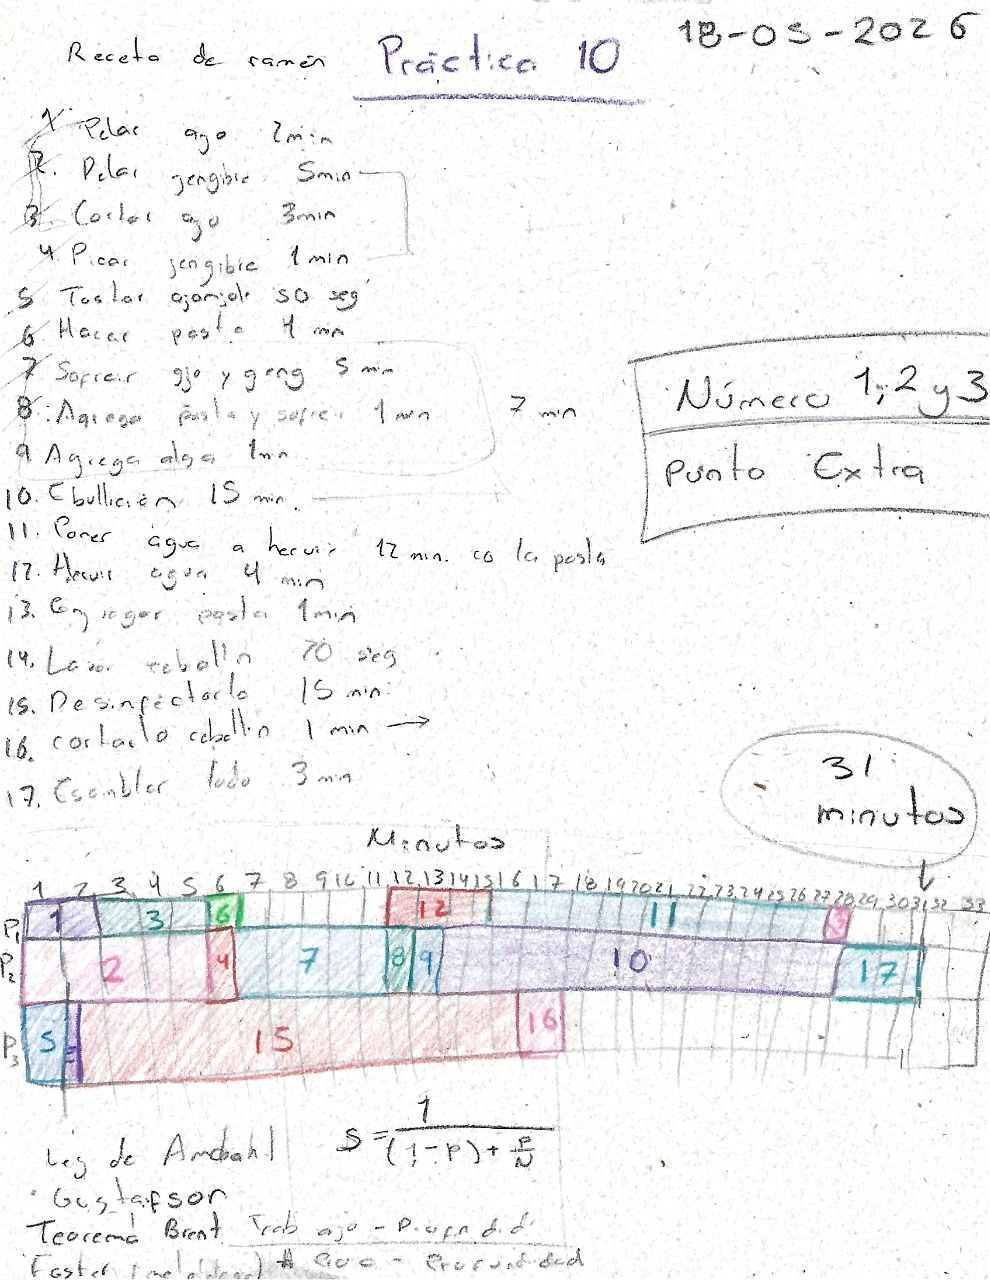
\includegraphics[width=\textwidth,height=0.9\textheight,keepaspectratio]{val-img.jpg}
\end{center}

\newpage

% ================================================================
\section*{Conclusiones}
% ================================================================

Esta práctica permitió comprender de manera más clara cómo funciona el procesamiento paralelo y por qué es tan importante en sistemas modernos y aplicaciones de tiempo real. A través de los distintos módulos fue posible observar que dividir correctamente las tareas entre varios núcleos puede mejorar considerablemente el rendimiento de un sistema, aunque también introduce nuevos retos relacionados con sincronización y acceso concurrente a recursos compartidos.\\

El ejercicio de la receta ayudó a entender conceptos como dependencias, balanceo de carga y camino crítico, mostrando cómo una correcta organización de tareas reduce el tiempo total de ejecución. De igual manera, los ejemplos de escalabilidad permitieron identificar cómo aparecen problemas como las condiciones de carrera y los cuellos de botella cuando varios procesos o trabajadores dependen de los mismos recursos o de un único punto de coordinación.\\

Además, el estudio del RP2040 permitió relacionar directamente la teoría con mecanismos reales de hardware, comprendiendo cómo funcionan las FIFOs para la comunicación entre núcleos y cómo los spinlocks ayudan a evitar colisiones cuando ambos núcleos intentan acceder al mismo recurso al mismo tiempo.

Finalmente, el caso del torno CNC mostró una aplicación práctica muy cercana a un entorno industrial real. La separación de tareas entre Core 0 y Core 1 permitió mantener la lectura continua del sensor mientras el otro núcleo realizaba operaciones lentas de impresión serial, evitando así la pérdida de muestras importantes.\\

En general, la práctica ayudó a reforzar y entender conceptos de concurrencia, paralelismo y sincronización, además de demostrar la importancia de diseñar sistemas eficientes y confiables para aplicaciones críticas en tiempo real.
\end{document}
